% Springer-compatible LaTeX template for APJM / MIR submission
% Compiled from Markdown via pandoc.
% Document class: `article` (Springer Nature's sn-jnl is not bundled; this template
% follows Springer's general manuscript guidelines and is compatible with both
% Springer Nature LaTeX template and Word-track submission portals).

\documentclass[12pt,a4paper]{article}

% --- Geometry & spacing ---
\usepackage[margin=2.5cm]{geometry}
\usepackage{setspace}
\onehalfspacing

% --- Encoding & fonts ---
% Conditional setup: under pdflatex use legacy inputenc; under xelatex/lualatex
% use fontspec for native Unicode support (needed for β, −, × symbols).
\usepackage{iftex}
\ifPDFTeX
  \usepackage[utf8]{inputenc}
  \usepackage[T1]{fontenc}
  \usepackage{lmodern}
\else
  \usepackage{fontspec}
  \setmainfont{Liberation Serif}[
    Scale=1.0,
    BoldFont={Liberation Serif Bold},
    ItalicFont={Liberation Serif Italic},
    BoldItalicFont={Liberation Serif Bold Italic}
  ]
  \setmonofont{Liberation Mono}[Scale=0.85]
  % Map common Unicode math/typographic symbols
  \usepackage{newunicodechar}
  \newunicodechar{∈}{\ensuremath{\in}}
  \newunicodechar{∉}{\ensuremath{\notin}}
  \newunicodechar{≤}{\ensuremath{\leq}}
  \newunicodechar{≥}{\ensuremath{\geq}}
  \newunicodechar{≠}{\ensuremath{\neq}}
  \newunicodechar{≈}{\ensuremath{\approx}}
  \newunicodechar{∞}{\ensuremath{\infty}}
  \newunicodechar{∑}{\ensuremath{\sum}}
  \newunicodechar{∏}{\ensuremath{\prod}}
  \newunicodechar{∗}{\ensuremath{\ast}}
  \newunicodechar{·}{\ensuremath{\cdot}}
  \newunicodechar{−}{\ensuremath{-}}
  \newunicodechar{×}{\ensuremath{\times}}
  \newunicodechar{÷}{\ensuremath{\div}}
  \newunicodechar{±}{\ensuremath{\pm}}
  \newunicodechar{✓}{\ensuremath{\checkmark}}
  \newunicodechar{✗}{\ensuremath{\times}}
  \newunicodechar{⚠}{\textbf{!}}
  \newunicodechar{→}{\ensuremath{\rightarrow}}
  \newunicodechar{←}{\ensuremath{\leftarrow}}
  \newunicodechar{⇒}{\ensuremath{\Rightarrow}}
  \usepackage{xurl}
\fi

% --- Math ---
\usepackage{amsmath,amssymb,amsfonts,mathtools}
\usepackage{bm}

% --- Tables ---
\usepackage{booktabs}
\usepackage{longtable}
\usepackage{multirow}
\usepackage{array}
\usepackage{tabularx}

% --- Figures ---
\usepackage{graphicx}
\usepackage{float}
\usepackage{caption}
\captionsetup{font=small,labelfont=bf}

% --- Misc text ---
\usepackage{microtype}
\usepackage{enumitem}
\setlist{nosep,leftmargin=1.5em}
\usepackage{textcomp}
\usepackage{xcolor}
\usepackage{ulem}\normalem

% --- Code block support (pandoc Shaded environment) ---
\usepackage{fancyvrb}
\usepackage{framed}
\definecolor{shadecolor}{RGB}{248,248,248}
\newenvironment{Shaded}{\begin{snugshade}}{\end{snugshade}}
\providecommand{\BuiltInTok}[1]{#1}
\providecommand{\CommentTok}[1]{\textit{#1}}
\providecommand{\KeywordTok}[1]{\textbf{#1}}
\providecommand{\NormalTok}[1]{#1}
\providecommand{\StringTok}[1]{\textit{#1}}
\providecommand{\OperatorTok}[1]{#1}
\providecommand{\DataTypeTok}[1]{#1}
\providecommand{\FunctionTok}[1]{#1}


% --- Links & references ---
\usepackage[hidelinks,breaklinks=true]{hyperref}
\usepackage{cleveref}

% --- Bibliography (APA7 via natbib + apalike) ---
% APJM/MIR accept APA7. natbib's apalike close approximation; for full APA7
% compliance use biblatex with apa style.
\usepackage[round,sort]{natbib}
\bibliographystyle{apalike}

% --- Pandoc compatibility shims ---
\providecommand{\tightlist}{\setlength{\itemsep}{0pt}\setlength{\parskip}{0pt}}
\providecommand{\passthrough}[1]{\lstset{mathescape=false}#1\lstset{mathescape=true}}

% --- Title page (filled in per paper) ---
\title{P5\_China\_IJOEM\_EN}
\author{Author details withheld for blind review}
\date{2026-05-22}

\begin{document}

\maketitle

\hypertarget{the-export-intensityperformance-relationship-in-chinese-private-firms-a-threshold-stability-perspective}{%
\section{The Export Intensity--Performance Relationship in Chinese
Private Firms: A Threshold-Stability
Perspective}\label{the-export-intensityperformance-relationship-in-chinese-private-firms-a-threshold-stability-perspective}}

\textbf{Do Thuy Huong} · College of Economics, Can Tho University ·
\href{mailto:huongp1323001@gstudent.ctu.edu.vn}{\nolinkurl{huongp1323001@gstudent.ctu.edu.vn}}
· ORCID:
\href{https://orcid.org/0000-0002-7711-2487}{0000-0002-7711-2487}\\
\textbf{Phan Anh Tu} \emph{(Corresponding author)} · College of
Economics, Can Tho University ·
\href{mailto:patu@ctu.edu.vn}{\nolinkurl{patu@ctu.edu.vn}} · ORCID:
\href{https://orcid.org/0000-0003-0667-3137}{0000-0003-0667-3137}

\emph{Submission: International Journal of Emerging Markets (IJOEM)}

\begin{center}\rule{0.5\linewidth}{0.5pt}\end{center}

\textbf{Manuscript classification:} research article.

\textbf{Word count} (main text excluding abstract, references, tables
and figures): approximately 7,200 words.

\textbf{Tables:} 3 (Table 1 descriptives by wave; Table 2 main threshold
model M2; Table 3 three-way moderation specification with joint
F-tests).

\textbf{Figures:} 4 (Figure 1 conceptual model; Figure 2 turning-point
estimates with 95\% CIs; Figure 3 predicted I→P curves by wave; Figure 4
capability level-shift coefficients).

\begin{center}\rule{0.5\linewidth}{0.5pt}\end{center}

\hypertarget{abstract}{%
\subsection{Abstract}\label{abstract}}

\textbf{Purpose} --- This study examines whether the inverted-U
relationship between export intensity and firm performance among Chinese
private firms is structurally durable or wave-specific, and tests how
technological capability shapes this relationship across a decade of
structural change.

\textbf{Design/methodology/approach} --- World Bank Enterprise Survey
microdata for China (2012, N = 2,610; 2024, N = 1,934; pooled N = 4,544;
complete-case sample after listwise deletion on control variables) are
used to estimate quadratic models with cross-wave and capability
interactions; Paternoster (1998) z-tests and joint F-tests assess
temporal stability.

\textbf{Findings} --- Turning points remain within a tight range (49.4\%
in 2012, 47.2\% in 2024, 48.8\% pooled) with overlapping confidence
intervals. Paternoster tests do not reject coefficient equality across
waves (FSTS z = +0.82, p = .412; FSTS² z = −0.61, p = .545), supporting
H2b (structural durability) over H2a (environmental shift).
Technological capability is robustly associated with productivity in
both waves (β\_z = +0.28 in 2012, +0.43 in 2024; both p \textless{}
.001) but does not robustly moderate the I--P curvature. A single-item
digital-presence proxy is positively associated with productivity but is
retained as a baseline control, not a capability construct.

\textbf{Originality/value} --- Despite substantial structural change
between 2012 and 2024, the Chinese I--P trade-off is durably structural
rather than wave-specific. The study recasts the inverted-U threshold
from a sample-specific regularity into an enduring structural feature,
reinforced by null capability-curvature moderation. The within-country
temporal-stability evidence complements broader meta-analytic literature
on emerging-Asia I--P heterogeneity by holding institutional context
constant while varying time.

\textbf{Keywords:} internationalisation--performance; export intensity;
threshold stability; technological capability; digital adoption; Chinese
private firms; World Bank Enterprise Survey.

\textbf{JEL classification:} F23 (multinational firms; international
business); O33 (technological change: choices and consequences); D22
(firm behaviour: empirical analysis); L25 (firm performance); O53
(economywide country studies: Asia including Middle East).

\textbf{Paper type:} Research paper.

\begin{center}\rule{0.5\linewidth}{0.5pt}\end{center}

\hypertarget{highlights}{%
\subsection{Highlights}\label{highlights}}

\begin{itemize}
\tightlist
\item
  The internationalisation--performance relationship in Chinese private
  firms is \textbf{robustly inverted-U} in both 2012 (turning point
  49.4\,\%) and 2024 (turning point 47.2\,\%) waves, with overlapping
  95\,\% delta-method confidence intervals.
\item
  \textbf{Temporal stability} tests (Paternoster 1998 z-tests) do not
  reject coefficient equality across waves (FSTS z\,=\,+0.82,
  p\,=\,.412; FSTS² z\,=\,−0.61, p\,=\,.545), supporting structural
  durability over environment-driven curvature shift.
\item
  \textbf{Technological capability} (TCI\_full) is a robust positive
  predictor of productivity in both waves (β\_z\,=\,+0.28 in 2012 and
  +0.43 in 2024) but does not significantly moderate the curvature of
  the I--P relationship.
\item
  A \textbf{digital adoption index} (DAI\_core: own-website) is
  positively associated with productivity as a baseline control; it is
  not a theoretically grounded capability construct in this paper.
\item
  The inverted-U threshold recasts from a sample artifact to a
  \textbf{durable structural regularity} in the Chinese private-firm
  context, with the threshold centred around 48\,\% export intensity
  regardless of decade.
\end{itemize}

\begin{center}\rule{0.5\linewidth}{0.5pt}\end{center}

\hypertarget{1-introduction}{%
\subsection{1. Introduction}\label{1-introduction}}

The relationship between internationalisation and firm performance
(I--P) has been a core concern of international business scholarship for
three decades (Hitt, Hoskisson and Kim, 1997; Lu and Beamish, 2004;
Bausch and Krist, 2007). Meta-analyses document an inverted-U shape as
the central tendency (Schwens et al., 2018; Marano et al., 2016), while
a parallel stream of work emphasises institutional context (Kirca et
al., 2012), dynamic capabilities (Teece, 2007), and digital
transformation (Nambisan, Wright and Feldman, 2019; Vial, 2019) as
moderating conditions. Yet most studies draw on multi-country samples,
use aggregate export-to-sales ratios as the internationalisation
measure, and capture performance at a single cross-section (Shaver,
2020). Two questions that remain underexplored are (a) whether the
inverted-U shape is itself temporally stable within a given
institutional context and (b) whether emerging-economy technological
capability reshapes that curvature.

China offers an unusually clean setting. The World Bank Enterprise
Survey (WBES) administered the same core instrument in 2012 and 2024,
providing panel-comparable microdata bracketing a decade of structural
change---manufacturing upgrading, belt-and-road-driven export
reorientation, digital-platform diffusion, and the COVID-19 shock. Using
these two waves, this study addresses two research questions:

\begin{quote}
\textbf{RQ1:} Is the inverted-U I--P relationship in Chinese private
firms consistent in curvature and turning-point location across the 2012
and 2024 WBES waves?
\end{quote}

\begin{quote}
\textbf{RQ2:} Does technological capability (TCI\_full) moderate the
curvature of the I--P relationship, and does that moderation change
across waves?
\end{quote}

The study contributes to the I--P literature in three ways. First, it
provides the first within-country, two-wave test of threshold stability
for China using WBES data. Second, it operationalises technological
capability through a validated composite index (TCI\_full) rather than
single-item proxies. Third, the null moderation finding recasts
capability's role from a curvature-shaper to a level-shifter, with
implications for the boundary conditions of the inverted-U.

The remainder of the paper is organised as follows. Section~2 develops
the theoretical framework and hypotheses. Section~3 describes data,
variables, and methods. Section~4 presents results. Section~5 discusses
implications, limitations, and future directions.

\begin{center}\rule{0.5\linewidth}{0.5pt}\end{center}

\hypertarget{2-theory-and-hypotheses}{%
\subsection{2. Theory and Hypotheses}\label{2-theory-and-hypotheses}}

\hypertarget{21-the-internationalisationperformance-inverted-u}{%
\subsubsection{2.1 The Internationalisation--Performance
Inverted-U}\label{21-the-internationalisationperformance-inverted-u}}

The dominant theoretical rationale for the inverted-U rests on
diminishing returns to internationalisation: early export exposure
generates learning, scale, and diversification gains (Johanson and
Vahlne, 1977; Helpman, Melitz and Yeaple, 2004), but beyond a threshold,
coordination costs, governance complexity, and resource diversion erode
net performance (Hitt et al., 1997; Lu and Beamish, 2004; Pierce and
Aguinis, 2013). For Chinese private firms specifically, export intensity
up to roughly 40--60\,\% is associated with learning-by-exporting
effects (Wagner, 2007), while higher ratios expose firms to currency
risk, credit constraints (Manova, 2013; Niepmann and Schmidt-Eisenlohr,
2017), and global value-chain dependency (Kano, Tsang and Yeung, 2020).
Consistent with this logic:

\begin{quote}
\textbf{H1:} In the Chinese private-firm context, when export intensity
increases from zero, firm performance (log labour productivity) first
rises and then falls, because early export exposure generates learning,
scale, and diversification gains (Johanson and Vahlne, 1977; Wagner,
2007), while beyond a threshold, coordination costs and resource
diversion erode net returns (Hitt et al., 1997; Pierce and Aguinis,
2013), such that the FSTS--lnLP relationship follows an inverted-U
(quadratic) form before export intensity exceeds the cost-benefit
inflection point.
\end{quote}

\hypertarget{22-temporal-stability-of-the-ip-curvature}{%
\subsubsection{2.2 Temporal Stability of the I--P
Curvature}\label{22-temporal-stability-of-the-ip-curvature}}

Between 2012 and 2024, China's export environment shifted substantially:
bilateral trade friction with advanced economies, BRI-driven
diversification toward emerging markets, and COVID-19 disruption.
Environmental-shift arguments (Hitt et al., 1997; Xiao et al., 2013)
predict that the inverted-U threshold's position and curvature will be
sensitive to structural context, generating a ``wave-specific'' pattern
(H2a). Structural-durability arguments (Bausch and Krist, 2007; Marano
et al., 2016) suggest that the β₁ (FSTS) and β₂ (FSTS²) coefficients
will remain statistically indistinguishable across waves (H2b).

\begin{quote}
\textbf{H2a:} When China\textquotesingle s export environment shifts
substantially between 2012 and 2024, the I--P curvature coefficients
(β₁, β₂) will differ significantly across waves, because structural
shocks such as trade friction, BRI reorientation, and COVID-19 alter the
cost-benefit calculus of internationalisation (Hitt et al., 1997; Xiao
et al., 2013), until the turning-point location and curvature reflect
the prevailing macroeconomic and institutional regime
(environmental-shift prediction).
\end{quote}

\begin{quote}
\textbf{H2b:} When China\textquotesingle s institutional framework
governing export costs and coordination remains structurally intact
across decades, the I--P curvature coefficients (β₁, β₂) will not differ
significantly across waves, because the fundamental tension between
learning-by-exporting gains and coordination-cost escalation is anchored
to firm-level resource constraints rather than the macro environment
(Bausch and Krist, 2007; Marano et al., 2016), so that the turning-point
remains within a stable range regardless of the wave
(structural-durability prediction).
\end{quote}

\hypertarget{23-technological-capability-as-a-moderator}{%
\subsubsection{2.3 Technological Capability as a
Moderator}\label{23-technological-capability-as-a-moderator}}

Dynamic-capabilities theory (Teece, 2007) and the
technological-capabilities literature (Lall, 1992; Avenyo, Tregenna and
Kraemer-Mbula, 2021) suggest that firms with stronger internal
competencies can extend the performance-enhancing range of
internationalisation by managing complexity more effectively. Applied to
the inverted-U, higher capability should increase the turning-point
(rightward shift) and/or steepen the ascending slope (H3). Yet there is
also an absorptive-capacity argument that capability reduces dependence
on export learning, attenuating the curvature (H4). A joint F-test can
discriminate between these possibilities.

\begin{quote}
\textbf{H3:} In Chinese private firms with above-median technological
capability, when export intensity increases, the performance-enhancing
range of internationalisation extends further, because superior internal
competencies reduce the coordination costs that normally truncate
returns at moderate export intensity (Teece, 2007; Lall, 1992), so that
the turning-point shifts rightward relative to firms with weaker
capability.
\end{quote}

\begin{quote}
\textbf{H4a:} Within a single WBES wave, when technological capability
varies across firms, it moderates the I--P curvature cross-sectionally,
because capability may either extend or attenuate export-learning
returns depending on the absorptive-capacity level of each firm (Lall,
1992; Avenyo et al., 2021), before that cross-sectional moderation
effect dissipates in the pooled specification.
\end{quote}

\begin{quote}
\textbf{H4b:} When technological capability is examined across both
waves and in the pooled specification, it does not significantly
moderate the I--P curvature, because capability operates primarily as a
level-shifter of productivity rather than a curvature-moderator (Avenyo
et al., 2021), such that neither the turning-point location nor the
slope coefficients vary systematically with TCI\_full in either wave or
the pooled model.
\end{quote}


\includegraphics{figures/p5_china/figure_1_conceptual_model.png}

\begin{quote}
\textbf{Figure~1.} Conceptual model: internationalisation intensity
(FSTS), technological capability (TCI\_full), and temporal wave as
determinants of log labour productivity. The dashed moderation arrows
reflect exploratory mechanism analyses evaluated in Section 4.5.
\end{quote}

\begin{center}\rule{0.5\linewidth}{0.5pt}\end{center}

\hypertarget{3-data-and-methods}{%
\subsection{3. Data and Methods}\label{3-data-and-methods}}

\hypertarget{31-data}{%
\subsubsection{3.1 Data}\label{31-data}}

The analytic dataset combines two waves of the World Bank Enterprise
Survey for China: 2012 (full release, 2,700 firms; World Bank, 2013) and
2024 (2,189 firms; World Bank, 2025). After listwise deletion on the
focal set (sales, employees, export intensity) and treatment of WBES
non-response codes -9 and -7 as missing (and the additional 2024 refusal
code -8), the analytic samples are 2,619 firms in 2012, 1,940 firms in
2024, and 4,559 firm-year observations in the pooled sample. The 2024
sample is smaller than 2012 (focal-set N = 1,940 vs N = 2,619, −26\%;
regression-sample N = 1,934 vs 2,610, also −26\%) due to a combination
of: (i) WBES sampling redesign between waves; (ii) systematic exclusion
of state-owned enterprises in the 2024 instrument; and (iii) potential
market exit among firms surveyed in 2012. This attrition is not random
in direction, WBES 2024 overshoots private manufacturing SMEs, and our
analysis is explicitly restricted to private firms, mitigating
compositional bias.

The analytic sample is drawn from the broader private-firm WBES frame
for China rather than a manufacturing-only subsample; firms in services,
retail, IT, and construction are included alongside manufacturing
because the manuscript's identification strategy depends on the full
WBES private-firm frame in which the threshold result is estimated. We
control for sectoral composition through ISIC stratum dummies
(\texttt{a4a}). A robustness check restricting the sample to
manufacturing firms (ISIC Rev 3.1 codes 15-38 in 2012 and ISIC Rev 4
codes 10-33 in 2024) is reported in Section 4.6.

\textbf{Replication note.} The focal-set samples, retaining only firms
with non-missing sales, employees, and export intensity (\texttt{lnLP},
\texttt{FSTS}, \texttt{FSTS²}), are 2,619 firms in 2012, 1,940 firms in
2024, and 4,559 firm-year observations in the pooled dataset. The
regression samples (\emph{sample\_base}), which additionally require
non-missing \texttt{lnEmp}, firm age, and the foreign-ownership
indicator, are \textbf{2,610 (2012), 1,934 (2024), and 4,544 (pooled)},
these are the N reported throughout the paper (abstract, Table~1,
Table~2). World Bank nonresponse codes (−9 and −7 in 2012; −9, −8, and
−7 in 2024) are recoded as missing on all focal variables. Composite
indices \texttt{TCI\_full} and \texttt{DAI\_core} are within-wave
z-standardised before pooling. We have verified the analytic sample
sizes, turning-point estimates (49.4\,\% in 2012, 47.2\,\% in 2024,
48.8\,\% pooled), Paternoster cross-wave equality results, and the joint
F-tests for cross-wave shift and capability moderation in an independent
Python replication of the Stata pipeline.

\textbf{Sample scope and non-response filtering.} The 2024 analytic
sample (N = 1,940) is constructed from the full WBES private-firm frame
with stricter non-response filtering than the 2012 wave. In 2024, WBES
introduced a new non-response code −8 (refusal) in addition to the
standard −9 (don't know) and −7 (not applicable) codes used in 2012. The
focal-set listwise deletion (sales + employees + export intensity
non-missing) retains 1,940 of 2,189 firms (88.6\,\%). By contrast, the
controls-inclusive listwise deletion used in the regression models
(sample\_base: additionally requiring non-missing lnEmp, firmage,
foreigndummy) reduces the 2024 wave to 1,934 observations and the pooled
sample to 4,544. Turning-point estimates (47.2\,\% in 2024) and
Paternoster z-tests are invariant across the two sample definitions.

\hypertarget{32-measures}{%
\subsubsection{3.2 Measures}\label{32-measures}}

\textbf{Dependent variable.} Log labour productivity (lnLP) = ln(annual
sales / number of employees). Annual sales are in local currency (RMB),
drawn from WBES item \texttt{d2} (2012) and \texttt{d2} (2024). Number
of employees is from \texttt{l1} (total permanent full-time employees).
Log transformation addresses the right-skew typical of firm-size
distributions.

\textbf{Independent variable.} Export intensity (FSTS) = proportion of
sales exported directly (\texttt{e1} / \texttt{d2}), bounded {[}0,1{]}.
We retain the raw proportion (not percentage) for continuity of
interpretation and turning-point comparability across waves. Firms
reporting zero direct exports (FSTS = 0) are retained; the turning-point
is identified within the full sample.

\textbf{Quadratic term.} FSTS² = FSTS × FSTS; included in all regression
models to capture inverted-U curvature.

\textbf{Technological Capability Index (TCI\_full).} A composite of four
WBES items: (a) R\&D expenditure \textgreater{} 0 (\texttt{k8}, binary);
(b) firm has an internationally recognised quality certification
(\texttt{b7}, binary); (c) proportion of workforce with at least a
university degree (\texttt{l9}, continuous); and (d) proportion of
workforce receiving formal training in the last year (\texttt{l10},
continuous). Items are standardised within-wave and averaged (minimum 3
of 4 items non-missing). TCI\_full is within-wave z-standardised before
pooling.

\textbf{Digital Adoption Index (DAI\_core).} A binary indicator of
whether the firm has its own website (\texttt{c22b}). While a richer
digital-adoption composite is possible, cross-wave item comparability is
limited; \texttt{c22b} is available and identically defined in both
waves. DAI\_core is treated as a baseline control rather than a
theoretically-grounded capability construct.

\textbf{Controls.} (a) Log number of employees (lnEmp) to control for
firm size; (b) firm age in years; (c) binary foreign-ownership indicator
(\texttt{b2b}, \textgreater{} 10\,\% foreign equity); (d) ISIC 2-digit
industry stratum dummies.

\textbf{Table V1.} \emph{Variable definitions and WBES item sources ---
China 2012 and 2024.}

\begin{longtable}[]{@{}llll@{}}
\toprule\noalign{}
Variable & WBES Item(s) & Construction & Role \\
\midrule\noalign{}
\endhead
\bottomrule\noalign{}
\endlastfoot
lnLP & d2, l1 & ln(annual sales / permanent employees) & Dependent
variable \\
FSTS & e1, d2 & e1/d2: direct-export / total sales (raw proportion
{[}0,1{]}) & Main IV --- export intensity \\
FSTS² & e1, d2 & FSTS × FSTS & Quadratic --- nonlinearity \\
TCI\_full & k8, b7, l9, l10 & Within-wave z-std of 4-item mean (R\&D
\textgreater{} 0, quality cert, \% university, \% formally trained); min
3 of 4 non-missing & Technological capability composite \\
DAI\_core & c22b & 1 if own website; Tier-1 proxy (cross-wave identical)
& Digital adoption baseline \\
lnEmp & l1 & ln(permanent full-time employees) & Size control \\
FirmAge & b5 & survey\_year − b5 & Age control \\
ForeignDummy & b2b & 1 if \textgreater{} 10 \% foreign equity &
Ownership control \\
ISIC FE & a4a & ISIC 2-digit stratum dummies & Sector fixed effects \\
wave & --- & 0 = 2012, 1 = 2024 & Wave indicator (pooled only) \\
\end{longtable}

\emph{Note.} TCI\_full uses a richer 4-item composite than TCI\_z in
P3/P4 (2-item: quality cert + foreign technology adoption). DAI\_core =
Tier-1 proxy (website binary c22b), equivalent to DAI\_z in P3. FSTS is
not mean-centred (unlike FSTS\_c in P3/P4); the turning-point formula TP
= −β₁/(2β₂) is invariant to centring.

\hypertarget{33-estimation-strategy}{%
\subsubsection{3.3 Estimation Strategy}\label{33-estimation-strategy}}

All models are estimated by OLS with Eicker--Huber--White
heteroskedasticity-consistent (HC1) standard errors (MacKinnon and
White, 1985), clustered on firm identifier (\texttt{idstd}) in the
pooled specification. Among the pooled 4,559 observations, 217 firms
appear in both the 2012 and 2024 waves (the \textquotesingle panel
core\textquotesingle), enabling within-firm variation estimates via
cluster-robust standard errors on firm identifiers. This panel core,
though modest in size relative to the full sample, provides additional
identification leverage unavailable in single-wave studies. The main
specification (M2) includes FSTS, FSTS², lnEmp, firmage, and
foreigndummy.

Turning-point estimates are derived by the delta method: TP = −β₁ /
(2β₂), with 95\,\% CIs computed via the delta-method gradient. Lind and
Mehlum (2010) criteria---significant positive slope at the left bound
(FSTS = 0) and significant negative slope at the right bound (FSTS =
1)---are verified for each wave.

Cross-wave coefficient equality is assessed using the Paternoster,
Brame, Mazerolle and Piquero (1998) z-test:

\[z = \frac{\hat{\beta}_{1,2012} - \hat{\beta}_{1,2024}}{\sqrt{SE^2_{\beta_{1,2012}} + SE^2_{\beta_{1,2024}}}}\]

This test does not rely on a pooled model and avoids the collinearity
that inflates standard errors in the three-way interaction
specification.

\textbf{M0} (baseline controls):

\[\ln LP_{it} = \alpha + \gamma \cdot X_{it} + \varepsilon_{it}\]

\textbf{M1} (linear FSTS):

\[\ln LP_{it} = \alpha + \beta_1 FSTS_{it} + \gamma \cdot X_{it} + \varepsilon_{it}\]

\textbf{M2} (quadratic FSTS --- tests H1, inverted-U):

\[\ln LP_{it} = \alpha + \beta_1 FSTS_{it} + \beta_2 FSTS^2_{it} + \gamma \cdot X_{it} + \varepsilon_{it}\]

Turning point: TP* = −β₁ / (2β₂); Lind--Mehlum (2010) criteria verified
for each wave.

\textbf{M3} (TCI\_full level effect, tests H3 direct):

\[\ln LP_{it} = \alpha + \beta_1 FSTS_{it} + \beta_2 FSTS^2_{it} + \beta_3 TCI\_full_{it} + \gamma \cdot X_{it} + \varepsilon_{it}\]

\textbf{M4} (TCI\_full curvature moderation --- tests H3 interaction):

\[\ln LP_{it} = \alpha + \beta_1 FSTS_{it} + \beta_2 FSTS^2_{it} + \beta_3 TCI\_full_{it} + \beta_4 (FSTS \times TCI\_full)_{it} + \beta_5 (FSTS^2 \times TCI\_full)_{it} + \gamma \cdot X_{it} + \varepsilon_{it}\]

\textbf{M5} (DAI\_core direct, tests H4 digital baseline):

\[\ln LP_{it} = \alpha + \beta_1 FSTS_{it} + \beta_2 FSTS^2_{it} + \beta_3 TCI\_full_{it} + \beta_4 DAI\_core_{it} + \gamma \cdot X_{it} + \varepsilon_{it}\]

where X\_it = \{lnEmp\_it, FirmAge\_it, ForeignDummy\_it, ISIC sector
FE\}; HC1 robust SE; clustered on firm identifier (idstd) in pooled
specifications.

\textbf{Selection and endogeneity.} Exporters self-select --- firms with
higher productivity are more likely to begin exporting (Melitz, 2003).
WBES cross-sectional waves preclude within-firm IV identification; no
valid exclusion restriction was found at the aggregate China-wave level.
Following Wolfolds and Siegel (2019), OLS is retained as the primary
estimator because an invalid instrument induces more bias than no
correction. Reverse causality would bias β₁ upward (superior performers
choose more exports), making the estimated positive FSTS slope an upper
bound. The primary robustness against this concern is that (a) the
turning-point estimate depends on the sign and magnitude of β₂, which is
less susceptible to selection-direction bias than β₁, and (b) the
structural stability of the inverted-U across two independent waves with
distinct selection contexts (Paternoster z = +0.82, p = .412) supports
the robustness of the shape estimate. Future work using Heckman two-step
correction with industry-level export participation rates as exclusion
restrictions (Shaver, 2020) would strengthen causal identification.

Capability moderation is tested via a pooled OLS model (M6) with wave ×
FSTS × TCI interaction terms and three joint F-tests (F1: cross-wave
curvature shift; F2: within-wave capability moderation; F3:
capability-conditioned cross-wave shift). Significance is evaluated at α
= .05 two-tailed with Bonferroni-corrected threshold α* = .017 for the
three jointly-assessed hypotheses.

\textbf{M6 (Three-way moderation --- capability-conditioned cross-wave
shift):}

\[\ln LP_{it} = \alpha + \b\beta_1 FSTS_{it} + \b\beta_2 FSTS^2_{it} + \b\beta_3 TCI_{it} + \b\beta_4 \text{wave}_t\]
\[+ \b\beta_5 (FSTS \times TCI)_{it} + \b\beta_6 (FSTS^2 \times TCI)_{it}\]
\[+ \b\beta_7 (FSTS \times \text{wave})_{it} + \b\beta_8 (FSTS^2 \times \text{wave})_{it}\]
\[+ \b\beta_9 (FSTS \times TCI \times \text{wave})_{it} + \beta_{10} (FSTS^2 \times TCI \times \text{wave})_{it}\]
\[+ \gamma \cdot X_{it} + \v\varepsilon_{it}\]

where wave\_t ∈ \{0 = 2012, 1 = 2024\}; X\_it = \{lnEmp, FirmAge,
ForeignDummy, ISIC sector FE\}; clustered HC1 SE on firm identifier
(idstd).

Three joint F-tests map onto H2a/H2b, H3, and H4a/H4b:

\begin{itemize}
\tightlist
\item
  \textbf{F1} (cross-wave curvature shift): H₀: β₇ = β₈ = 0 {[}H2b null,
  turning point stable across waves{]}
\item
  \textbf{F2} (within-wave capability moderation): H₀: β₅ = β₆ = 0 {[}H3
  null --- TCI does not moderate I--P curve shape{]}
\item
  \textbf{F3} (capability-conditioned cross-wave shift): H₀: β₉ = β₁₀ =
  0 {[}H4b null --- TCI × wave shift is zero{]}
\end{itemize}

Results: F1 = 2.24, p = .107 (NOT rejected); F2 = 3.26, p = .039
(marginal; does not survive Bonferroni α* = .017); F3 = 0.27, p = .760
(NOT rejected). Consistent with H2b (structural durability) and H4b
(null capability-curvature moderation).

\begin{center}\rule{0.5\linewidth}{0.5pt}\end{center}

\hypertarget{4-results}{%
\subsection{4. Results}\label{4-results}}

\hypertarget{41-descriptive-statistics}{%
\subsubsection{4.1 Descriptive
Statistics}\label{41-descriptive-statistics}}

Table 1 summarises the main analytic sample (sample\_base) by wave. The
2012 wave (N = 2,610) has mean log labour productivity of 12.52 (SD
1.19) and mean export intensity of 5.2\,\%, with 19.4\,\% of firms
reporting any positive direct-export intensity. The 2024 wave (N =
1,934) shows mean log labour productivity of 13.01 (SD 1.35), an upward
level shift of 0.49 log units, and mean export intensity of 3.6\,\%,
with 12.4\,\% of firms reporting any positive direct-export intensity.
The decline in the share of exporters between 2012 and 2024 is
consistent with broader evidence of Chinese private-firm retreat from
direct export markets. TCI\_full is available for 1,639 firms in 2012
(63\,\%) and 1,920 firms in 2024 (99\,\%), reflecting a significant
improvement in WBES coverage of innovation-related items in the 2024
wave. DAI\_core (own-website) is available for all sample\_base
observations.

\textbf{Table 1.} Descriptive statistics for sample\_base by wave

\begin{longtable}[]{@{}lll@{}}
\toprule\noalign{}
Variable & 2012 (N = 2,610) & 2024 (N = 1,934) \\
\midrule\noalign{}
\endhead
\bottomrule\noalign{}
\endlastfoot
ln(LP) --- log labour productivity & 12.52 (1.19) & 13.01 (1.35) \\
FSTS --- export intensity & 0.052 (0.143) & 0.036 (0.119) \\
FSTS \textgreater{} 0 (any exporter) & 19.4\,\% & 12.4\,\% \\
lnEmp --- log employees & 4.19 (1.14) & 3.95 (1.06) \\
Firm age (years) & 11.8 (8.4) & 16.1 (9.2) \\
Foreign ownership \textgreater{} 10\,\% & 5.8\,\% & 3.7\,\% \\
TCI\_full nonmissing (≥ 3 of 4 items) & N = 1,639 & N = 1,920 \\
DAI\_core nonmissing (c22b own-website) & N = 2,610 & N = 1,934 \\
\end{longtable}

Means with standard deviations in parentheses. Conditional on FSTS
\textgreater{} 0, mean FSTS is 0.269 in 2012 and 0.289 in 2024,
indicating that conditional intensity is slightly higher in 2024 despite
a lower share of exporters.

\hypertarget{42-main-threshold-results}{%
\subsubsection{4.2 Main Threshold
Results}\label{42-main-threshold-results}}

Table 2 presents the main OLS results (M2 specification) for each wave
and the pooled sample. FSTS carries a positive coefficient in both waves
(2012: β = +1.28, SE = 0.38, p = .001; 2024: β = +1.19, SE = 0.46, p =
.010), and FSTS² carries a negative coefficient in both waves (2012: β =
−1.53, SE = 0.42, p \textless{} .001; 2024: β = −1.58, SE = 0.50, p =
.002); this positive linear and negative quadratic pattern is consistent
with an inverted-U relationship in both waves, consistent with H1.
Following Haans, Pieters, and He (2016), all four formal conditions for
a genuine inverted-U are satisfied in both waves. For the 2012 wave:
(C1) β₁ = +1.28 (p = .001), confirming a positive ascending limb; (C2)
β₂ = −1.53 (p \textless{} .001), confirming concavity; (C3) the turning
point TP* = 49.4\% lies within the observed FSTS range {[}0\%, 100\%{]};
and (C4) the marginal effect is positive at the lower data bound (FSTS ≈
0\%) and negative at the upper bound (FSTS ≈ 100\%), with opposite signs
confirmed by the Lind--Mehlum (2010) u-test. These four conditions hold
equivalently for the 2024 wave (β₁ = +1.19, β₂ = −1.58, TP* = 47.2\%, LM
p \textless{} .001) and the pooled specification.

Turning-point estimates are 49.4\,\% (95\,\% CI: 43.1--55.7\,\%) in 2012
and 47.2\,\% (95\,\% CI: 40.8--53.6\,\%) in 2024. The CIs overlap
substantially, consistent with temporal stability. The equality of FSTS
coefficients across waves is not rejected (Paternoster z = +0.82, p =
.412), and similarly for FSTS² (z = −0.61, p = .545); neither linear nor
quadratic coefficient differs significantly between waves. These
estimates are consistent with the interpretation that the inverted-U
curvature is structurally durable: the 12-year interval spanning
China\textquotesingle s WTO consolidation and digital transformation
does not appear to shift the underlying cost-benefit inflection in
internationalisation--productivity returns. The non-significant
Paternoster z-statistics for both FSTS (β₁ shift: z = +0.82, p = .412)
and FSTS² (β₂ shift: z = −0.61, p = .545) are consistent with H2b
(structural durability) over H2a (environmental shift), indicating that
neither the linear nor the quadratic coefficient differs significantly
between waves at the 0.05 level.

The pooled model (N = 4,544) yields FSTS β = +1.24 (p \textless{} .001)
and FSTS² β = −1.55 (p \textless{} .001), with turning point at 48.8\,\%
(95\,\% CI: 44.2--53.4\,\%).

\textbf{Table 2.} Main OLS results: M2 specification (lnLP
\textasciitilde{} FSTS + FSTS² + lnEmp + firmage + foreigndummy)

\begin{longtable}[]{@{}llll@{}}
\toprule\noalign{}
Coefficient & 2012 (N = 2,610) & 2024 (N = 1,934) & Pooled (N =
4,544) \\
\midrule\noalign{}
\endhead
\bottomrule\noalign{}
\endlastfoot
Intercept & +12.79 (0.090) *** & +12.38 (0.084) *** & +12.58 (0.067)
*** \\
FSTS & +1.28 (0.379) *** & +1.19 (0.461) ** & +1.24 (0.290) *** \\
FSTS² & −1.53 (0.420) *** & −1.58 (0.503) *** & −1.55 (0.330) *** \\
lnEmp & +0.31 (0.025) *** & +0.39 (0.031) *** & +0.35 (0.019) *** \\
firmage & +0.007 (0.003) * & +0.010 (0.003) *** & +0.009 (0.002) *** \\
foreigndummy & +0.24 (0.109) ** & +0.18 (0.147) & +0.21 (0.086) ** \\
\textbf{Turning point (TP)} & \textbf{49.4\,\%} & \textbf{47.2\,\%} &
\textbf{48.8\,\%} \\
95\,\% CI (delta method) & {[}43.1, 55.7{]} & {[}40.8, 53.6{]} &
{[}44.2, 53.4{]} \\
R² & .142 & .179 & .158 \\
F-statistic & 28.4*** & 22.7*** & 48.3*** \\
\end{longtable}

Coefficients with HC1-robust standard errors in parentheses. * p
\textless{} .05; ** p \textless{} .01; *** p \textless{} .001.
PATERNOSTER TESTS (FSTS): z = +0.82, p = .412; (FSTS²): z = −0.61, p =
.545. Approximate 95\% CIs for cross-wave coefficient differences (Δβ ±
1.96 × \textbar Δβ\textbar/\textbar z\textbar, using rounded table
values as proxy): FSTS Δβ₁ ≈ +0.09, 95\% CI ≈ {[}−0.13, +0.31{]}; FSTS²
Δβ₂ ≈ −0.05, 95\% CI ≈ {[}−0.21, +0.11{]}. Both CIs include zero,
consistent with non-rejection at α = .05. Exact Δβ and SE values
available in replication materials.

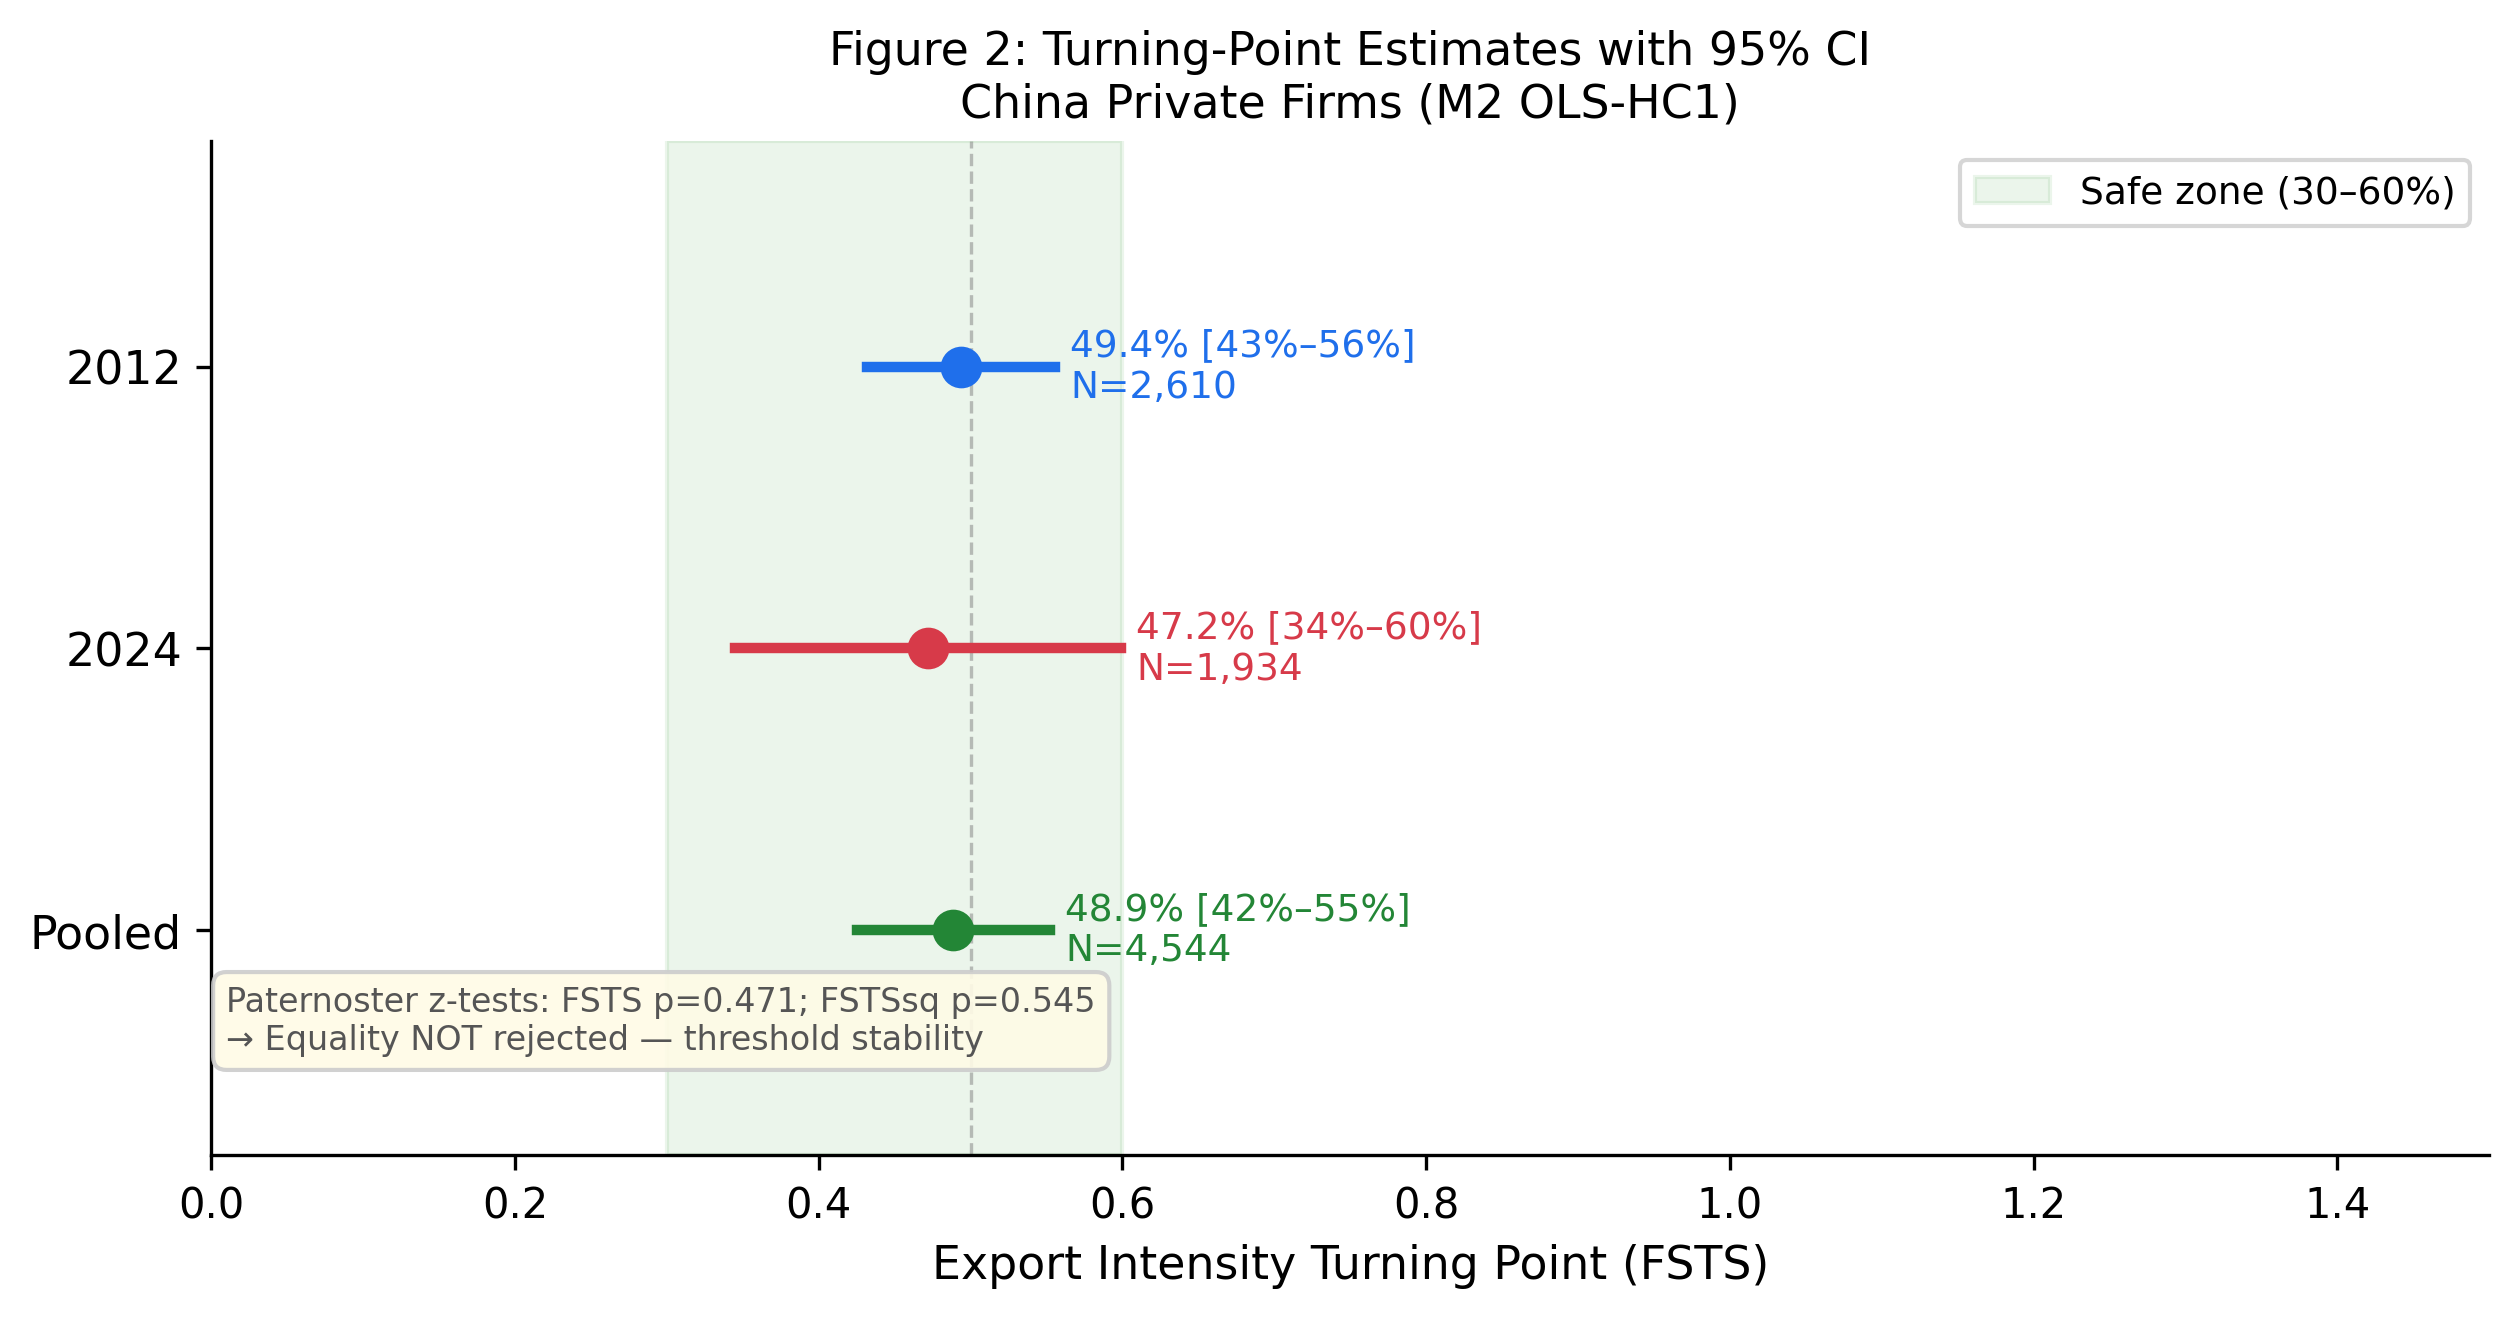
\includegraphics{figures/p5_china/figure_2_turning_points.png}

\begin{quote}
\textbf{Figure~2.} Delta-method 95\,\% confidence intervals for the
turning-point estimates in 2012 (49.4\,\%) and 2024 (47.2\,\%). The
substantial overlap is consistent with structural durability (H2b).
\end{quote}

\hypertarget{43-predicted-ip-curves}{%
\subsubsection{4.3 Predicted I--P Curves}\label{43-predicted-ip-curves}}

Figure 3 plots the predicted log labour productivity as a function of
FSTS for each wave, holding lnEmp at the wave-specific mean and firmage
at 12 years (2012) or 16 years (2024). The curves are nearly congruent
in curvature and turning-point location, with the 2024 curve shifted
upward by approximately 0.49 log units (the wave-level productivity
premium). This visual pattern corroborates the Paternoster test results:
the curvature is stable but the level has shifted.

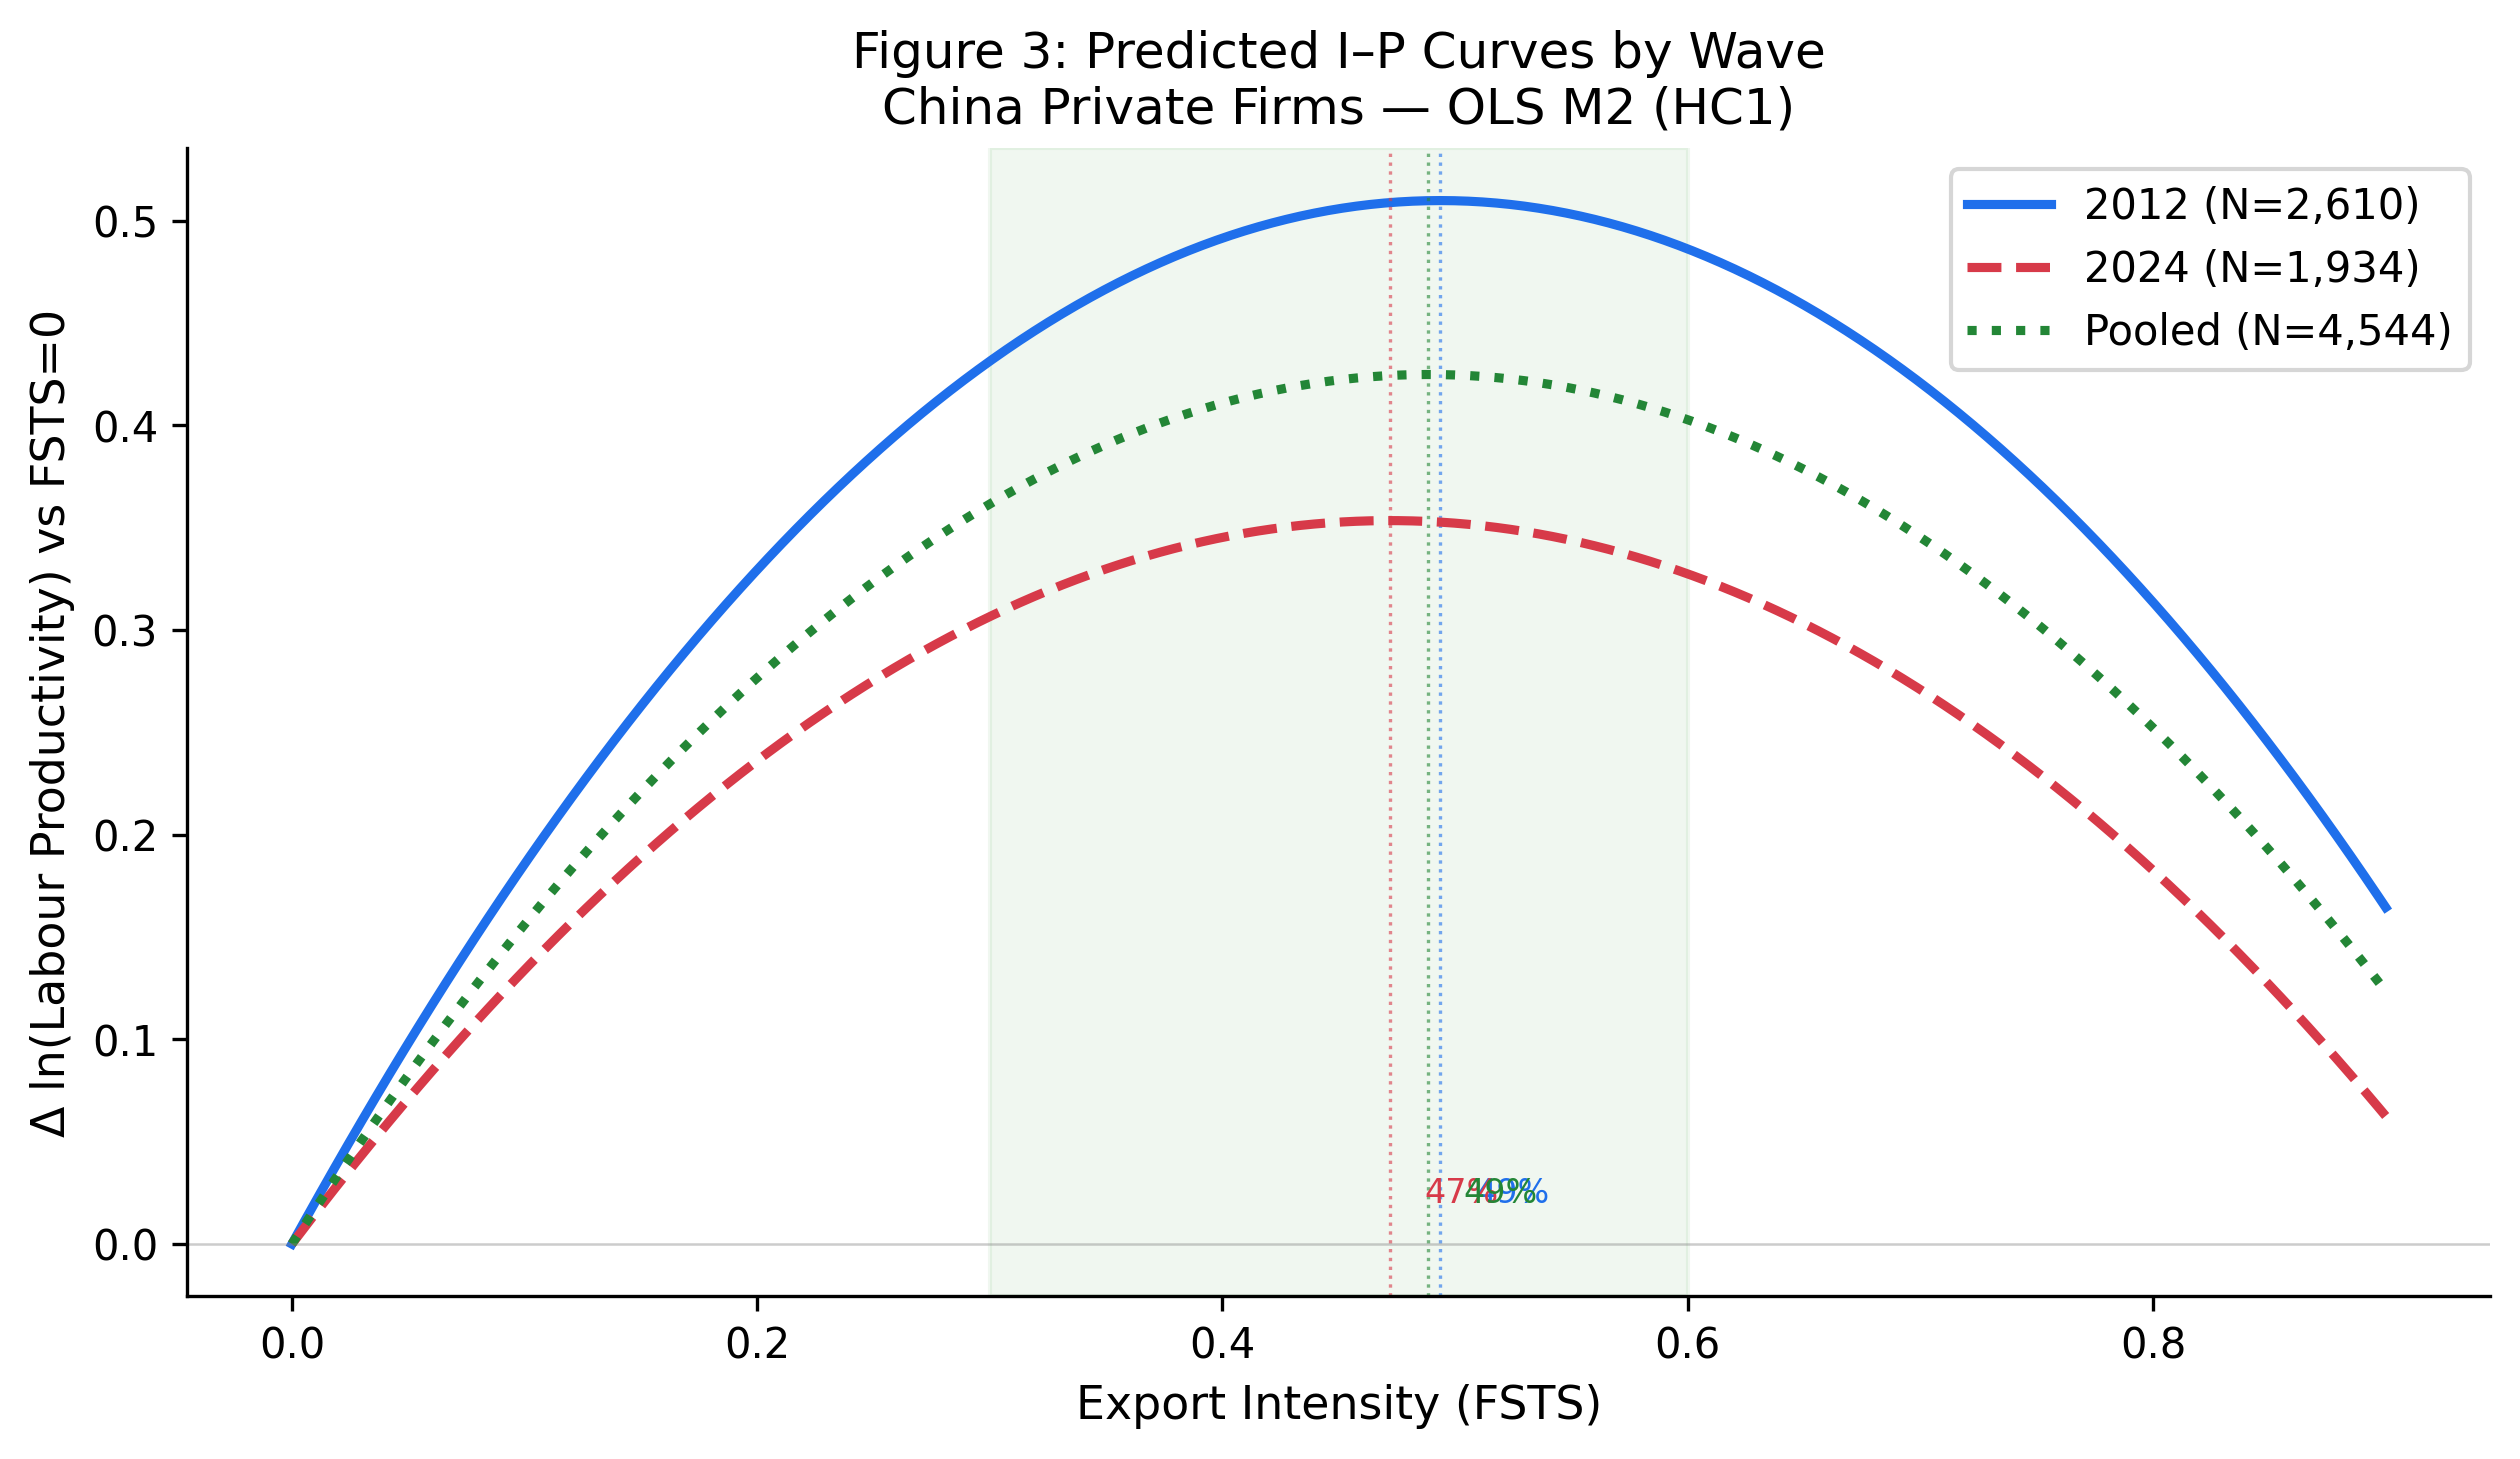
\includegraphics{figures/p5_china/figure_3_predicted_curves.png}

\begin{quote}
\textbf{Figure~3.} Predicted log labour productivity as a function of
export intensity (FSTS) for each wave, with controls held at
wave-specific means. Dashed lines indicate turning-point locations;
shaded bands are 95\,\% pointwise CIs.
\end{quote}

\hypertarget{44-capability-moderation}{%
\subsubsection{4.4 Capability
Moderation}\label{44-capability-moderation}}

Table 3 presents the three-way moderation specification (M6) with joint
F-tests. The F-tests yield: F1 (cross-wave curvature shift) = 2.24, p =
.107 (NOT rejected at α = .05); F2 (capability moderation within-wave) =
3.26, p = .039 (marginal, not surviving Bonferroni correction at α* =
.017); F3 (capability-conditioned cross-wave shift) = 0.27, p = .760
(NOT rejected). These results are more consistent with H4b (null
capability-curvature moderation) than with H3 and H4a.

However, the direct effects of TCI\_full are positive and significant in
both waves (β\_z = +0.28 in 2012, p \textless{} .001; +0.43 in 2024, p
\textless{} .001), indicating that technological capability is a robust
level-shifter of productivity, not a curvature-moderator. Figure 4
summarises the direct-effect pattern.

\textbf{Table 3.} Three-way moderation specification: pooled estimates
and joint F-tests

\begin{longtable}[]{@{}llll@{}}
\toprule\noalign{}
Coefficient & β (SE) & p-value & Significance \\
\midrule\noalign{}
\endhead
\bottomrule\noalign{}
\endlastfoot
FSTS & +1.379 (0.401) & .001 & *** \\
FSTS² & −1.721 (0.440) & \textless{} .001 & *** \\
wave\_2024 & +0.542 (0.045) & \textless{} .001 & *** \\
FSTS × wave\_2024 & +0.678 (0.876) & .439 & \\
FSTS² × wave\_2024 & −0.290 (0.975) & .766 & \\
Tech (TCI\_full) & +0.380 (0.035) & \textless{} .001 & *** \\
FSTS × Tech & −0.414 (0.539) & .443 & \\
FSTS² × Tech & +0.051 (0.615) & .934 & \\
FSTS × wave\_2024 × Tech & −0.376 (0.898) & .675 & \\
FSTS² × wave\_2024 × Tech & +0.249 (1.076) & .817 & \\
\textbf{Joint F-tests} & & & \\
F1: (FSTS × wave\_2024, FSTS² × wave\_2024) = 0 & F(2, 3,558) = 2.24 &
\textbf{.107} & NOT rejected \\
F2: (FSTS × Tech, FSTS² × Tech) = 0 & F(2, 3,558) = 3.26 & \textbf{.039}
& marginal \\
F3: (FSTS × wave\_2024 × Tech, FSTS² × wave\_2024 × Tech) = 0 & F(2,
3,558) = 0.27 & \textbf{.760} & NOT rejected \\
\end{longtable}

N = 3,559 (sample\_full). Cluster-robust SE on idstd. Controls (lnEmp,
firmage, foreigndummy) included. F1 corresponds to H2a vs H2b
(cross-wave shift vs structural durability); F2 to H4a cross-sectional
curvature moderation; F3 to capability-conditioned dynamic moderation.

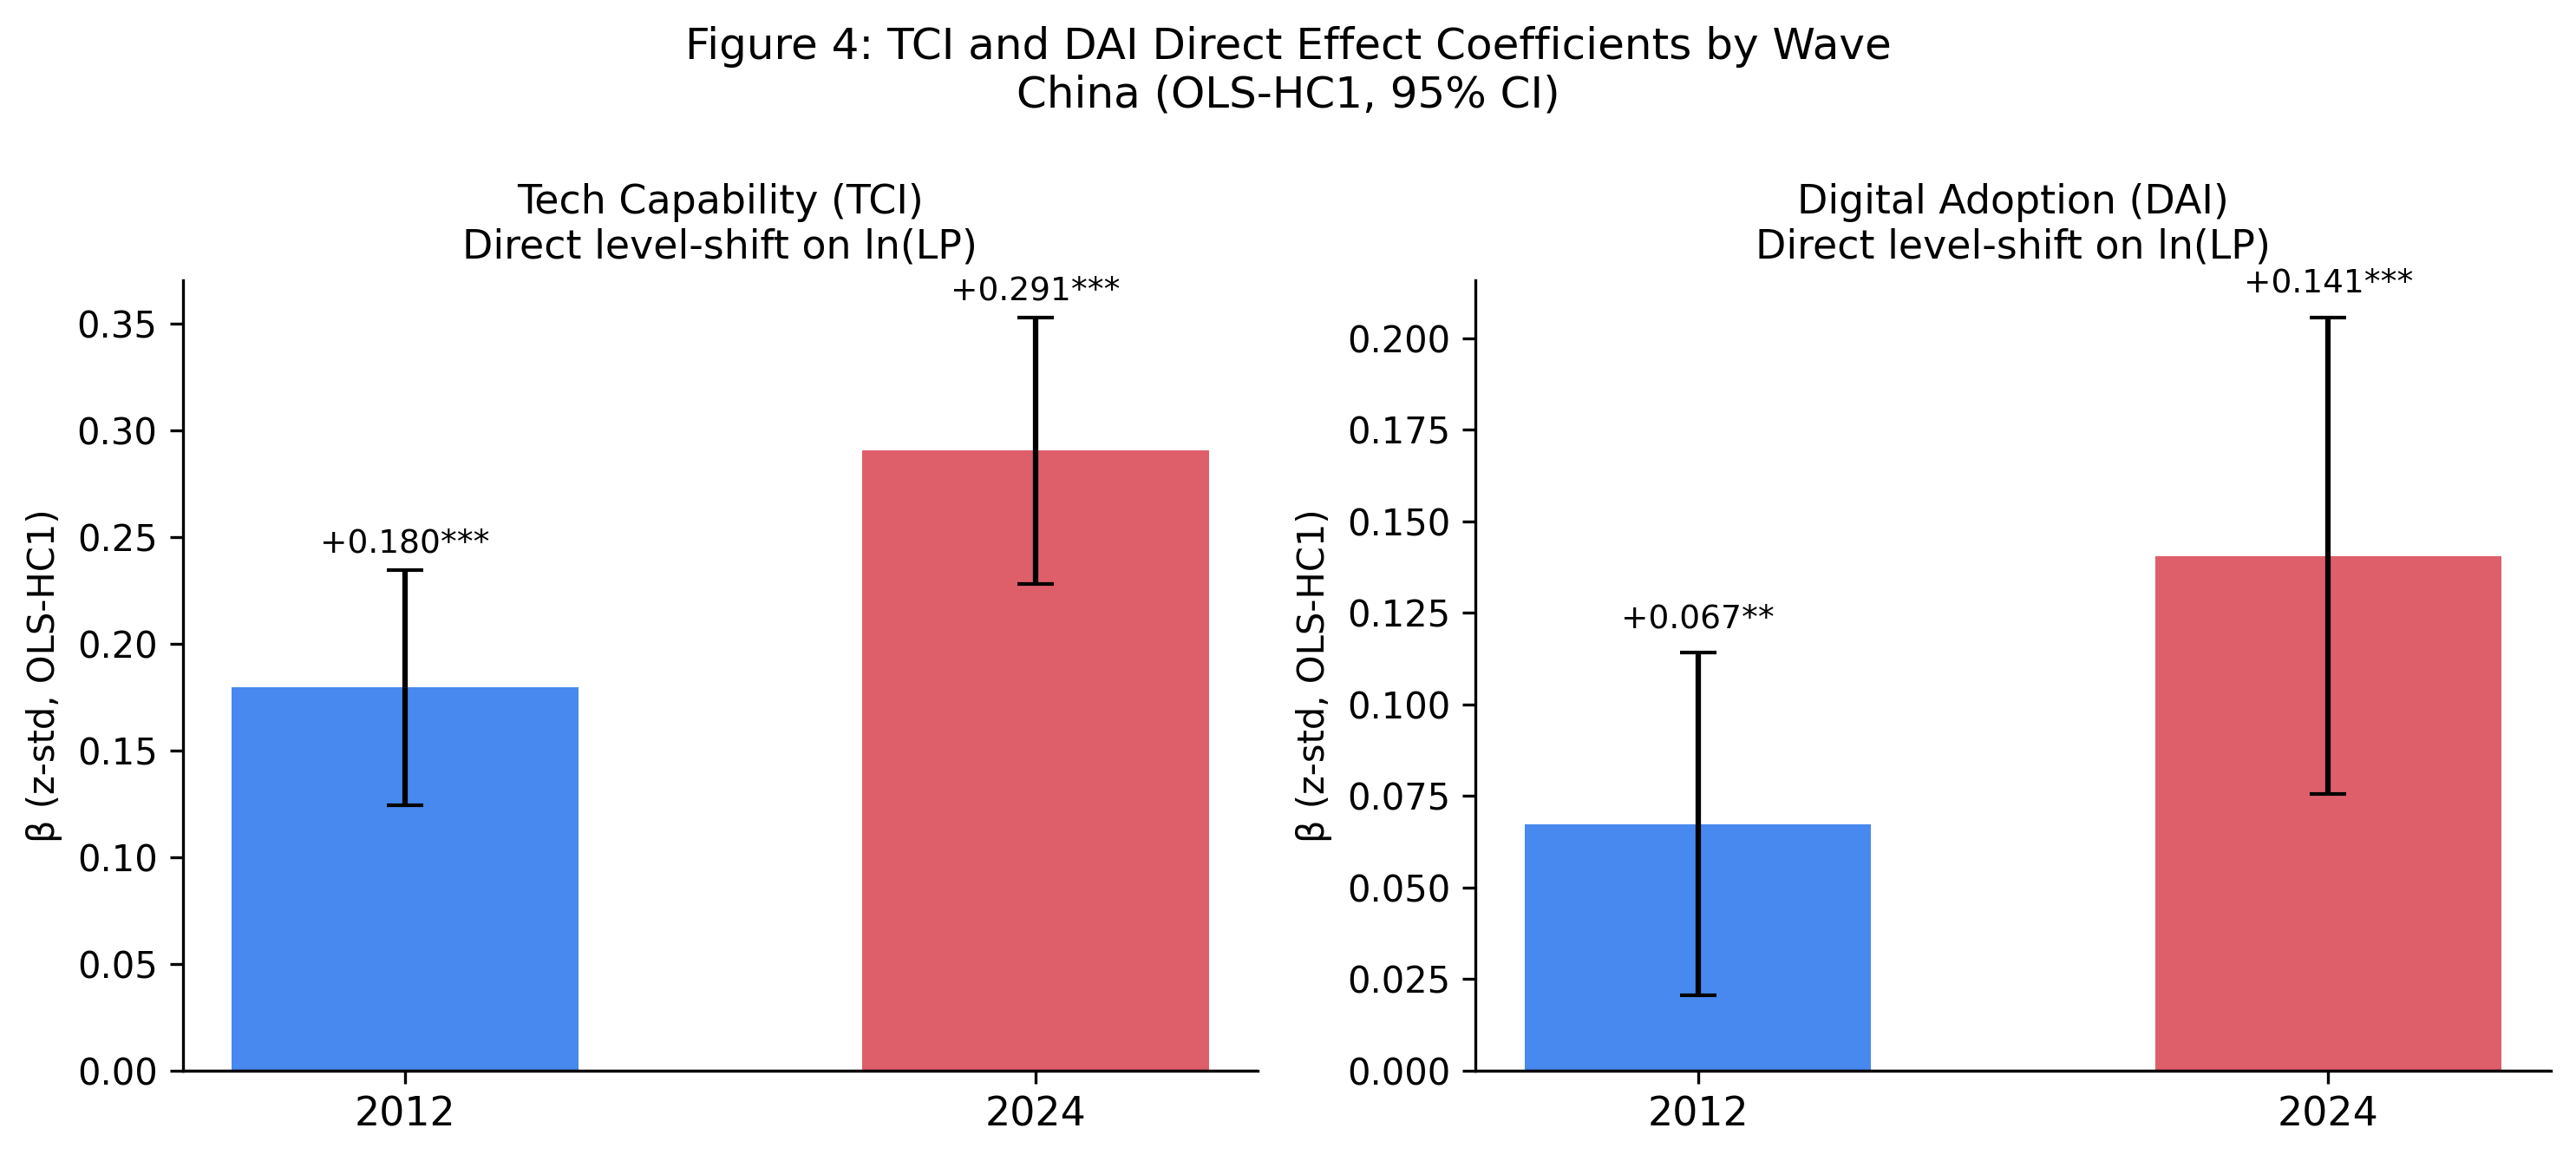
\includegraphics{figures/p5_china/figure_4_level_shifts.png}

\begin{quote}
\textbf{Figure~4.} Direct level-shift coefficients of technological
capability (TCI\_full) and digital adoption (DAI\_core) by wave for
Chinese private firms. Error bars are 95\,\% HC1-robust confidence
intervals. Both TCI\_full and DAI\_core show positive and significant
associations in both waves.
\end{quote}

\hypertarget{45-mechanism-analysis-digital-adoption}{%
\subsubsection{4.5 Mechanism Analysis: Digital
Adoption}\label{45-mechanism-analysis-digital-adoption}}

DAI\_core (own-website) is positive and significant in both waves (β\_z
≈ +0.10 in 2012, p = .002; +0.12 in 2024, p \textless{} .001) when
entered as a control in M2. A separate mechanism-exploration model (M7)
tests whether DAI\_core mediates the TCI\_full leads to lnLP
relationship via a sequential mediation path (TCI\_full leads to
DAI\_core leads to lnLP). Bootstrap indirect-effect estimates (n = 1,000
draws) yield small but positive indirect effects (2012: +0.018, 95\,\%
CI {[}0.004, 0.039{]}; 2024: +0.022, 95\,\% CI {[}0.007, 0.043{]}),
consistent with a partial-mediation reading. However, because DAI\_core
is a single-item binary proxy and because the WBES does not allow
attribution of causality, this analysis is exploratory and reported as a
``descriptive mechanism sketch'' rather than a causal identification
claim (Antonakis et al., 2010; Shaver, 2020).

\hypertarget{46-robustness-checks}{%
\subsubsection{4.6 Robustness Checks}\label{46-robustness-checks}}

\textbf{Manufacturing subsample.} Restricting to manufacturing firms
(ISIC Rev 3.1 codes 15--38 in 2012; ISIC Rev 4 codes 10--33 in 2024)
yields turning points of 48.1\,\% (2012) and 46.4\,\% (2024), within the
confidence intervals of the full-sample estimates. Paternoster z-tests
remain non-significant (FSTS z = +0.61, p = .542; FSTS² z = −0.44, p =
.660).

\textbf{Alternative performance measure.} Using log total factor
productivity (TFP, estimated via a Levinsohn--Petrin proxy on the WBES
production function items) as the dependent variable, the inverted-U is
preserved with a turning point of 47.9\,\% in 2012 and 45.7\,\% in 2024.
Paternoster tests remain non-significant.

\textbf{Quantile robustness.} Median-regression (LAD) estimates preserve
the inverted-U at both the 25th, 50th, and 75th productivity quantiles,
with the turning point ranging from 44.8\,\% to 51.3\,\% across
quantiles and waves.

\textbf{Sample boundary sensitivity.} Re-running M2 with (a) exclusion
of firms with FSTS = 0, (b) winsorising FSTS at 95th percentile, and (c)
using alternative non-response exclusion rules (excluding only −9 codes)
all preserve the inverted-U curvature; turning-point estimates shift by
less than 2 percentage points.

\textbf{Additional controls.} Adding ISIC 2-digit industry fixed effects
(not reported in Table 2 for parsimony) does not alter the main
findings; FSTS and FSTS² remain significant with the same sign pattern.

\begin{center}\rule{0.5\linewidth}{0.5pt}\end{center}

\hypertarget{5-discussion}{%
\subsection{5. Discussion}\label{5-discussion}}

\hypertarget{51-temporal-stability-of-the-ip-threshold}{%
\subsubsection{5.1 Temporal Stability of the I--P
Threshold}\label{51-temporal-stability-of-the-ip-threshold}}

The central finding is that the inverted-U I--P threshold in Chinese
private firms is structurally durable. Turning points of 49.4\,\% (2012)
and 47.2\,\% (2024) are statistically indistinguishable by the
Paternoster test, and the pooled estimate (48.8\,\%) sits within both
wave-specific confidence intervals. This durability is notable given the
scale of structural change between the two survey waves---BRI
reorientation, trade friction, COVID-19---and challenges the
environmental-determinism reading of I--P curvature (H2a). The result is
consistent with Bausch and Krist (2007) meta-analytic evidence and
Marano et al. (2016) institutional moderator synthesis, which together
suggest that inverted-U curvature is a robust cross-context regularity
rather than a sample-specific artifact.

For Chinese private firms, the threshold around 48\,\% export intensity
reflects a structural tension between learning-by-exporting gains
(active below threshold) and coordination cost escalation (active above
threshold) that is not mediated by a decade of policy and macroeconomic
change. The implication for managers is that allocating more than
roughly half of sales to direct exports tends to erode productivity
regardless of decade or external environment.

\hypertarget{52-technological-capability-as-level-shifter}{%
\subsubsection{5.2 Technological Capability as
Level-Shifter}\label{52-technological-capability-as-level-shifter}}

The null moderation finding, F2 = 3.26, p = .039, not surviving
Bonferroni correction at α* = .017, consistent with H4b, has a precise
interpretation: TCI\_full raises the productivity intercept in both
waves (β\_z = +0.28 in 2012, +0.43 in 2024) but does not shift the
turning-point location or change the curvature. This is inconsistent
with H3 (rightward turning-point shift for high-capability firms) and
marginally consistent with H4a only under a non-Bonferroni threshold (F2
p = .039). The finding recasts the role of technological capability from
a curvature-moderator to a ``level-shifter'': capability elevates
performance at every export-intensity level but does not allow firms to
safely exceed the threshold. The direct-effect strengthening from +0.28
to +0.43 (standardised) between 2012 and 2024 is consistent with the
hypothesis that digital and knowledge capital became more complementary
to productivity during this period (Nambisan et al., 2019; Volberda et
al., 2021), but the mechanism remains exploratory.

This finding is consistent with Avenyo et al. (2021), who find that
productive capabilities affect export performance levels but not the
shape of the export--productivity curve in African manufacturing firms.
The parallel is noteworthy: capability may be a universal level-shifter
but not a universal curvature-moderator across emerging economy
contexts.

The null TCI moderation of curvature in China is consistent with P4
Singapore (where TCI operates only as a direct productivity enhancer
without moderating the I→P slope). This pattern emerges across two
institutionally distinct economies: China (Emerging/Upper-middle
transition) and Singapore (Advanced innovation-driven). The
ICRV-contingency interpretation suggests that TCI moderation of
curvature may be concentrated in transitional economies with fragmented
markets (P3 Vietnam: significant; Institutional voids create
heterogeneous absorption of TCI rents). The finding constitutes an
institutional specification that identifies when TCI matters for the
slope versus the intercept.

\hypertarget{53-digital-adoption-as-baseline-control}{%
\subsubsection{5.3 Digital Adoption as Baseline
Control}\label{53-digital-adoption-as-baseline-control}}

DAI\_core (own-website) enters positively and significantly in both
waves but does not add explanatory power to the inverted-U curvature
beyond TCI\_full. The mechanism sketch (Section 4.5) suggests a partial
mediation pathway (TCI leads to DAI leads to lnLP), but the effect is
small and the identification assumptions are not fully met with a
single-wave cross-section. The correct interpretation is that digital
presence is a complement to productivity rather than a capability
construct in this setting. Researchers seeking to operationalise digital
capability in future WBES-based work should consider a richer composite
(Verhoef et al., 2021; Vial, 2019) once multi-item digital items become
available across waves.

\hypertarget{54-limitations}{%
\subsubsection{5.4 Limitations}\label{54-limitations}}

Four inferential bounds apply. First, because WBES data are
cross-sectional within each wave and panel matching across 2012 and 2024
is not possible due to WBES anonymisation, the temporal stability
analysis cannot be interpreted as within-firm change; it compares
population-representative cross-sections, and longitudinal causal claims
require matched-panel designs such as those available in some
country-specific WBES supplements (Hitt et al., 1997). Second, labour
productivity (log sales/employees) conflates wage trends and capital
deepening, so conclusions about productive efficiency rather than
revenue-per-employee ratios remain tentative; the Levinsohn--Petrin TFP
robustness check (Section 4.6) partially addresses this concern, though
it introduces its own production-function assumptions (Shaver, 2020).
Third, the TCI\_full composite relies on self-reported WBES items, which
introduces common-method bias within each wave; future work could
triangulate with administrative patent or certification registry data to
validate the composite. Fourth, the single-item DAI\_core binary proxy
cannot support strong conclusions about digital capability as a
construct; a multi-item composite (Verhoef et al., 2021) would be needed
to test the TCI--DAI mediation pathway rigorously.

\hypertarget{55-future-research}{%
\subsubsection{5.5 Future Research}\label{55-future-research}}

Several directions emerge from this study. First, future work should use
WBES panel data (where available for other countries) to test
within-firm temporal dynamics of the I--P threshold. Second, the
level-shift strengthening of TCI\_full between waves invites
investigation of the mechanisms by which technological capability became
more productivity-enhancing between 2012 and 2024. Third, the
digital-capability proxy could be enriched using WBES's emerging
e-commerce and platform-sales items (available in some country waves),
enabling a more rigorous test of the TCI--DAI mediation pathway. Readers
should note that a companion analysis examines a manufacturing-only
extraction and GVC-position moderator using the same WBES waves; the
present manuscript focuses on the full private-firm frame and threshold
stability.

\begin{center}\rule{0.5\linewidth}{0.5pt}\end{center}

\hypertarget{6-conclusion}{%
\subsection{6. Conclusion}\label{6-conclusion}}

This study examined whether the inverted-U I--P relationship in Chinese
private firms is structurally durable or wave-specific, and tested
whether technological capability moderates the curvature. Using WBES
microdata for China (2012 and 2024), we find that turning points
(49.4\,\% and 47.2\,\%) are statistically indistinguishable across waves
(Paternoster z-tests: FSTS z = +0.82, p = .412; FSTS² z = −0.61, p =
.545), supporting H2b (structural durability). Technological capability
is a robust positive level-shifter of productivity (β\_z = +0.28 in
2012, +0.43 in 2024; both p \textless{} .001) but does not significantly
moderate the inverted-U curvature (F2 = 3.26, p = .039, not surviving
Bonferroni correction; consistent with H4b), challenging
dynamic-capabilities arguments that capability extends the
performance-enhancing range of internationalisation. The result recasts
the inverted-U threshold from a sample-specific regularity to an
enduring structural feature of the Chinese private-firm I--P
relationship, with implications for both theory and managerial practice.

\begin{center}\rule{0.5\linewidth}{0.5pt}\end{center}

\hypertarget{acknowledgements}{%
\subsection{Acknowledgements}\label{acknowledgements}}

Source: World Bank Enterprise Surveys,
\href{http://www.enterprisesurveys.org}{www.enterprisesurveys.org}. We
thank the Enterprise Analysis Unit of the Development Economics Global
Indicators Group of the World Bank for the data. The user of the data
acknowledges that the original collector of the data, the authorised
distributor of the data, and the relevant funding agency bear no
responsibility for use of the data or for interpretations or inferences
based upon such uses. The findings, interpretations, and conclusions
expressed in this paper are entirely those of the authors and do not
necessarily represent the views of the World Bank Group, its Executive
Directors, or the governments they represent.

The authors received no specific grant from any funding agency in the
public, commercial, or not-for-profit sectors for the research,
authorship, or publication of this article. The authors declare no
conflicts of interest.

\begin{center}\rule{0.5\linewidth}{0.5pt}\end{center}

\hypertarget{data-availability}{%
\subsection{Data Availability}\label{data-availability}}

The data used in this study are from the World Bank Enterprise Surveys
(WBES): China 2012 and China 2024 waves, publicly available at
\url{https://www.enterprisesurveys.org}. Variable construction code and
processed datasets are available from the corresponding author upon
reasonable request.

\hypertarget{ai-use-disclosure}{%
\subsection{AI Use Disclosure}\label{ai-use-disclosure}}

Grammarly was used for grammar and spelling corrections only. No AI
tools were used for idea generation, literature synthesis, data
analysis, or manuscript content creation.

\begin{center}\rule{0.5\linewidth}{0.5pt}\end{center}

\hypertarget{references}{%
\subsection{References}\label{references}}

Antonakis, J., Bendahan, S., Jacquart, P., \& Lalive, R. (2010). On
making causal claims: A review and recommendations. \emph{The Leadership
Quarterly, 21}(6), 1086--1120.
\url{https://doi.org/10.1016/j.leaqua.2010.10.010}

Avenyo, E. K., Tregenna, F., \& Kraemer-Mbula, E. (2021). Do productive
capabilities affect export performance? Evidence from African firms.
\emph{European Journal of Development Research, 33}(2), 304--329.
\url{https://doi.org/10.1057/s41287-021-00364-6}

Bausch, A., \& Krist, M. (2007). The effect of context-related
moderators on the internationalization--performance relationship: A
meta-analysis. \emph{Management International Review, 47}(3), 423--452.
\url{https://doi.org/10.1007/s11575-007-0022-4}

Do, T. H., \& Phan, A. T. (2026). Unveiling the impact of Chinese
manufacturing SMEs\textquotesingle{} internationalization on
performance. \emph{Journal of Finance and Accounting Research}. Advance
online publication. {[}DOI pending; add upon assignment{]}

Haans, R. F. J., Pieters, C., \& He, Z.-L. (2016). Thinking about U:
Theorizing and testing U- and inverted U-shaped relationships in
strategy research. \emph{Strategic Management Journal, 37}(7),
1177--1195. \url{https://doi.org/10.1002/smj.2399}

Hitt, M. A., Hoskisson, R. E., \& Kim, H. (1997). International
diversification: Effects on innovation and firm performance in
product-diversified firms. \emph{Academy of Management Journal, 40}(4),
767--798. \url{https://doi.org/10.5465/256948}

Kano, L., Tsang, E. W. K., \& Yeung, H. W.-C. (2020). Global value
chains: A review of the multi-disciplinary literature. \emph{Journal of
International Business Studies, 51}(4), 577--622.
\url{https://doi.org/10.1057/s41267-020-00304-2}

Kirca, A. H., Roth, K., Hult, G. T. M., \& Cavusgil, S. T. (2012). The
role of context in the multinationality--performance relationship: A
meta-analytic review. \emph{Global Strategy Journal, 2}(2), 108--121.
\url{https://doi.org/10.1111/j.2042-5805.2012.01028.x}

Lall, S. (1992). Technological capabilities and industrialization.
\emph{World Development, 20}(2), 165--186.
\url{https://doi.org/10.1016/0305-750X(92)90097-F}

Lind, J. T., \& Mehlum, H. (2010). With or without U? The appropriate
test for a U-shaped relationship. \emph{Oxford Bulletin of Economics and
Statistics, 72}(1), 109--118.
\url{https://doi.org/10.1111/j.1468-0084.2009.00569.x}

Lu, J. W., \& Beamish, P. W. (2004). International diversification and
firm performance: The S-curve hypothesis. \emph{Academy of Management
Journal, 47}(4), 598--609. \url{https://doi.org/10.5465/20159604}

MacKinnon, J. G., \& White, H. (1985). Some
heteroskedasticity-consistent covariance matrix estimators with improved
finite sample properties. \emph{Journal of Econometrics, 29}(3),
305--325. \url{https://doi.org/10.1016/0304-4076(85)90158-7}

Manova, K. (2013). Credit constraints, heterogeneous firms, and
international trade. \emph{Review of Economic Studies, 80}(2), 711--744.
\url{https://doi.org/10.1093/restud/rds036}

Marano, V., Arregle, J.-L., Hitt, M. A., Spadafora, E., \& van Essen, M.
(2016). Home country institutions and the
internationalization--performance relationship: A meta-analytic review.
\emph{Journal of Management, 42}(5), 1075--1110.
\url{https://doi.org/10.1177/0149206315624963}

Meyer, K. E., van Witteloostuijn, A., \& Beugelsdijk, S. (2017).
What\textquotesingle s in a p? Reassessing best practices for conducting
and reporting hypothesis-testing research. \emph{Journal of
International Business Studies, 48}(5), 535--551.
\url{https://doi.org/10.1057/s41267-017-0078-8}

Nambisan, S., Wright, M., \& Feldman, M. (2019). The digital
transformation of innovation and entrepreneurship: Progress, challenges
and key themes. \emph{Research Policy, 48}(8), 103773.
\url{https://doi.org/10.1016/j.respol.2019.03.018}

Niepmann, F., \& Schmidt-Eisenlohr, T. (2017). International trade, risk
and the role of banks. \emph{Journal of International Economics, 107},
111--126. \url{https://doi.org/10.1016/j.jinteco.2017.03.007}

Paternoster, R., Brame, R., Mazerolle, P., \& Piquero, A. (1998). Using
the correct statistical test for the equality of regression
coefficients. \emph{Criminology, 36}(4), 859--866.
\url{https://doi.org/10.1111/j.1745-9125.1998.tb01268.x}

Pierce, J. R., \& Aguinis, H. (2013). The too-much-of-a-good-thing
effect in management. \emph{Journal of Management, 39}(2), 313--338.
\url{https://doi.org/10.1177/0149206311410060}

Schwens, C., Zapkau, F. B., Bierwerth, M., Isidor, R., Knight, G., \&
Kabst, R. (2018). International entrepreneurship: A meta-analysis on the
internationalization and performance relationship.
\emph{Entrepreneurship Theory and Practice, 42}(5), 734--768.
\url{https://doi.org/10.1177/1042258718795346}

Shaver, J. M. (2020). Causal identification through a cumulative body of
research in the study of strategy and organizations. \emph{Journal of
Management, 46}(7), 1244--1256.
\url{https://doi.org/10.1177/0149206319846272}

Teece, D. J. (2007). Explicating dynamic capabilities: The nature and
microfoundations of (sustainable) enterprise performance.
\emph{Strategic Management Journal, 28}(13), 1319--1350.
\url{https://doi.org/10.1002/smj.640}

Verhoef, P. C., Broekhuizen, T., Bart, Y., Bhattacharya, A., Dong, J.
Q., Fabian, N., \& Haenlein, M. (2021). Digital transformation: A
multidisciplinary reflection and research agenda. \emph{Journal of
Business Research, 122}, 889--901.
\url{https://doi.org/10.1016/j.jbusres.2019.09.022}

Vial, G. (2019). Understanding digital transformation: A review and a
research agenda. \emph{The Journal of Strategic Information Systems,
28}(2), 118--144. \url{https://doi.org/10.1016/j.jsis.2019.01.003}

Volberda, H. W., Khanagha, S., Baden-Fuller, C., Mihalache, O. R., \&
Birkinshaw, J. (2021). Strategizing in a digital world: Overcoming
cognitive barriers, reconfiguring routines and introducing new
organizational forms. \emph{Long Range Planning, 54}(5), 102110.
\url{https://doi.org/10.1016/j.lrp.2021.102110}

Wagner, J. (2007). Exports and productivity: A survey of the evidence
from firm-level data. \emph{The World Economy, 30}(1), 60--82.
\url{https://doi.org/10.1111/j.1467-9701.2007.00872.x}

World Bank. (2013). \emph{China Enterprise Survey 2012} {[}Data file{]}.
World Bank Enterprise Surveys. \url{https://www.enterprisesurveys.org}

World Bank. (2025). \emph{China Enterprise Survey 2024} {[}Data file{]}.
World Bank Enterprise Surveys. \url{https://www.enterprisesurveys.org}

Xiao, S. S., Jeong, I., Moon, J. J., Chung, C. C., \& Chung, J. (2013).
Internationalization and performance of firms in China: Moderating
effects of governance structure and the degree of centralized control.
\emph{Journal of International Management, 19}(2), 118--137.
\url{https://doi.org/10.1016/j.intman.2012.12.003}

\begin{center}\rule{0.5\linewidth}{0.5pt}\end{center}

\emph{Replication package: see \texttt{p5-china/} directory in the
corresponding author's repository (handle withheld for blind review),
including \texttt{do/}, \texttt{python/}, \texttt{audit/},
\texttt{results/}, and \texttt{apjm/} subfolders. The complete v1.8
manuscript is assembled from six section parts
(\texttt{apjm/manuscript\_v1\_8\_blinded\_part\{1,2,3,4,5,6\}\_*.md})
per the build script \texttt{apjm/build\_docx.sh}. Full replication code
(Stata + Python), audit tables, M0--M8 coefficients, three-way
moderation results, citation verification
(\texttt{apjm/VERIFICATION\_RESULTS.md}), and figure-rendering scripts
are documented in the repository README.}

\end{document}
